%!TEX root = ../main.tex

\chapter{Diseño de hardware}
\label{ch:hardware}

Una vez definida la arquitectura general en el \cref{ch:arquitectura}, en este capítulo se aborda el diseño eléctrico y físico del sistema. Primero se presentan las decisiones tomadas respecto a los componentes, qué módulos se utilizan y por qué, y para cada módulo, qué modelo se ha seleccionado. Después se analiza el sistema de alimentación empleado, el esquema eléctrico con todos los componentes, el diseño de la PCB, la fabricación de la misma y, finalmente, las pruebas de verificación realizadas sobre el hardware. 

\section{Selección de componentes}
\label{sec:seleccion_componentes}

En esta sección se justifica la selección de cada componente del sistema, del nodo transmisor y del nodo receptor. Para cada categoría funcional definida en el \cref{ch:arquitectura}, se evalúan las opciones más relevantes disponibles actualmente en el mercado y se justifica la elección final en función de los requisitos, el coste, entre otros factores relevantes. 

Antes de empezar es importante resaltar que las categorías de sensores no se han elegido de forma arbitraria, sino que se derivan de los parámetros de vuelo requeridos para representar un PFD. La actitud y el rumbo magnético son el núcleo de una PFD, por lo que se requiere una unidad inercial y un magnetómetro. La altitud y la velocidad vertical, parámetros esenciales también, se obtienen de la presión atmosférica, por lo que se requiere de un barómetro. La velocidad respecto al suelo y la posición geográfica también son dos parámetros importantes si se quiere añadir un mapa de navegación, estos datos provienen de un receptor GNSS. La velocidad de suelo se emplea además como sustituto de la velocidad aerodinámica en el PFD, ya que la plataforma no incorpora sistema pitot-estático. La altura respecto al terreno o la detección de obstáculos también son parámetros relevantes. Para resolver este problema, se aborda desde dos perspectivas distintas, basadas en dos principios diferentes: el tiempo de vuelo y el radar FMCW. Así, no solo se obtienen dos parámetros comparables, sino que se puede contrastar ambas tecnologías con fines docentes. Por último, el enlace de telemetría inalámbrico entre los dos nodos requiere un transceptor de radiofrecuencia.


\subsection{Microcontroladores del transmisor y del receptor}
\label{sec:sel_mcu}

En el nodo transmisor se concentran todos los sensores y se ejecuta el firmware de fusión sensorial, por lo que idealmente se requiere procesado en coma flotante, memoria RAM suficiente y al menos dos UART hardware. El receptor solo
decodifica los paquetes recibidos y los reenvía por puerto serie virtual al
PC, por lo que los requisitos son mucho menos exigentes.

\begin{table}[H]
    \centering
    \caption{Alternativas evaluadas para los microcontroladores}
    \label{tab:sel_mcu}
    \footnotesize
    \begin{tabularx}{\linewidth}{L{2.1cm} C{1.2cm} C{1.3cm} C{0.7cm} C{1.4cm} X}
        \toprule
        \textbf{Modelo} & \textbf{RAM} & \textbf{Reloj} & \textbf{UART} & \textbf{Precio} & \textbf{Observaciones} \\
        \midrule
        Arduino Nano & 2 KB & 16 MHz & 1 & 3-5\,\euro{} & Un solo UART, sin FPU. \\
        STM32 F103 & 20 KB & 72 MHz & 3 & 3-6\,\euro{} & Buen rendimiento, sin radio. \\
        Raspberry Pi Pico & 264 KB & 133 MHz & 2 & 4\,\euro{} & Sin radio integrada. \\
        ESP32-S3 DevKit & 512 KB + 8 MB & 240 MHz & 3 & 6-8\,\euro{} & Seleccionado para el transmisor. \\
        ESP32-C3 Super Mini & 400 KB & 160 MHz & 2 & 3-4\,\euro{} & Seleccionado para el receptor. \\
        \bottomrule
    \end{tabularx}
\end{table}

El Arduino Nano queda descartado por su único UART hardware y por no
disponer de unidad de coma flotante, imprescindible para la fusión
sensorial. El STM32 F103 dispone de prestaciones suficientes, pero su RAM
es ajustada y su soporte en el ecosistema Arduino es menos maduro. El
Raspberry Pi Pico es una alternativa prometedora, pero, al igual que el STM32, carece de radio integrada y obligaría a un ecosistema distinto al del nodo receptor; a esta escala la diferencia de precio frente a la opción elegida es pequeña, por lo que se prefiere mantener un único entorno de desarrollo compartido por ambos nodos. Para el transmisor se
selecciona el ESP32-S3 DevKit \cite{ds_esp32s3} por sus tres
UART hardware, FPU, abundante memoria (\SI{512}{\kilo\byte} de RAM más
PSRAM) y un ecosistema Arduino IDE maduro. Para el receptor se elige el ESP32-C3 Super Mini \cite{ds_esp32c3}, ya que mantiene el mismo ecosistema con coste y tamaño menor. Sus dimensiones reducidas son perfectas para el receptor.

\subsection{Unidad de medida inercial y magnetómetro}
\label{sec:sel_imu}

La estimación de actitud y rumbo (RF01 y RF02) requiere una IMU que combine acelerómetro, giroscopio y magnetómetro, idealmente en un único módulo para hacer la implementación más sencilla.

\begin{table}[H]
    \centering
    \caption{Alternativas evaluadas para la unidad de medida inercial}
    \label{tab:sel_imu}
    \footnotesize
    \begin{tabularx}{\linewidth}{l c c c c X}
        \toprule
        \textbf{Modelo} & \textbf{Acel} & \textbf{Giro} & \textbf{Magn.} & \textbf{Precio} & \textbf{Observaciones} \\
        \midrule
        MPU-6050   & Sí & Sí & No & $\approx$3\,\euro{}  & Sin magnetómetro. \\
        MPU-9250   & Sí & Sí & Sí & $\approx$6\,\euro{}  & Seleccionado. \\
        ICM-20948  & Sí & Sí & Sí & $\approx$11\,\euro{} & Peor disponibilidad. \\
        LSM9DS1    & Sí & Sí & Sí & $\approx$13\,\euro{} & Librerías menos maduras. \\
        BNO055     & Sí & Sí & Sí & $\approx$22\,\euro{} & Fusión integrada en chip. \\
        \bottomrule
    \end{tabularx}
\end{table}

El MPU-6050 se descarta por no incorporar magnetómetro, lo que haría que se tuviese que utilizar un módulo independiente, lo cual es posible de implementar, pero se ha preferido descartar para este proyecto. El BNO055, aunque atractivo por integrar la fusión en el propio chip, no expone públicamente su algoritmo de fusión, lo que contradice el carácter docente del proyecto: se prefiere implementar la fusión explícitamente en firmware sobre datos sin manipular. Por este motivo, y por su coste muy superior, también se descarta. Las otras dos opciones se descartan por falta de disponibilidad y precio superior. Entre las restantes se selecciona el MPU-9250 \cite{ps_mpu9250}, que integra acelerómetro, giroscopio y,
conectado internamente por I2C, un magnetómetro AK8963 \cite{ds_ak8963}. Su biblioteca Arduino \cite{kriswiner_mpu9250} es la más madura del ecosistema. Aunque el fabricante ha discontinuado el MPU-9250, sigue siendo ampliamente disponible en el mercado de módulos \textit{breakout}, lo que no compromete la reproducibilidad de la plataforma (RC01).


\subsection{Sensor barométrico}
\label{sec:sel_baro}

El sensor barométrico cubre RF03 (altitud sobre el nivel del mar) y RF04
(velocidad vertical) mediante la presión atmosférica y la fórmula
barométrica de la atmósfera estándar \cite{icao_isa}.

\begin{table}[H]
    \centering
    \caption{Alternativas evaluadas para el sensor barométrico}
    \label{tab:sel_baro}
    \footnotesize
    \begin{tabularx}{\linewidth}{l c c c X}
        \toprule
        \textbf{Modelo} & \textbf{Precisión} & \textbf{Interface} & \textbf{Precio} & \textbf{Observaciones} \\
        \midrule
        BMP180  & $\pm 1$ m   & I2C       & $\approx$2\,\euro{}  & Obsoleto. \\
        BMP280  & $\pm 1$ m   & I2C / SPI & $\approx$3\,\euro{}  & Seleccionado. \\
        BME280  & $\pm 1$ m   & I2C / SPI & $\approx$4\,\euro{}  & Añade humedad, no requerida. \\
        BMP388  & $\pm 0{,}5$ m & I2C / SPI & $\approx$6\,\euro{}  & Mejor precisión, mayor coste. \\
        MS5611  & $\pm 0{,}1$ m & I2C / SPI & $\approx$9\,\euro{}  & Grado profesional. \\
        \bottomrule
    \end{tabularx}
\end{table}

Se selecciona el BMP280 \cite{ds_bmp280} por su balance entre precisión y precio. Ofrece precisión de ±1 m a un precio competitivo. El BMP180 está obsoleto, el BME280 es muy similar, pero añade un
sensor de humedad, que no es necesario en este contexto. La precisión superior del BMP388 y el
MS5611 no se traduce en mejora perceptible en este proyecto, así que no justifican el precio superior. La librería
de Adafruit \cite{lib_bmp280} del módulo seleccionado proporciona soporte robusto y la interfaz I2C se comparte con el MPU-9250.


\subsection{Receptor GNSS}
\label{sec:sel_gnss}

El receptor GNSS cubre RF05 (velocidad respecto al suelo) y proporciona la
posición geográfica para el mapa de navegación del PFD. RP05 fija la
precisión objetivo en \SI{2.5}{\meter} CEP.

\begin{table}[H]
    \centering
    \caption{Alternativas evaluadas para el receptor GNSS}
    \label{tab:sel_gnss}
    \footnotesize
    \begin{tabularx}{\linewidth}{l c c c X}
        \toprule
        \textbf{Modelo} & \textbf{Tasa max} & \textbf{Precisión CEP} & \textbf{Precio} & \textbf{Observaciones} \\
        \midrule
        NEO-6M   & 5 Hz  & 2,5 m & $\approx$10\,\euro{} & Seleccionado. \\
        NEO-M8N  & 10 Hz & 2,0 m & $\approx$14\,\euro{} & Mayor coste sin mejora perceptible. \\
        BN-880   & 10 Hz & 2,0 m & $\approx$20\,\euro{} & Brújula redundante con AK8963. \\
        ATGM336H & 10 Hz & 2,5 m & $\approx$8\,\euro{}  & Librerías menos maduras. \\
        \bottomrule
    \end{tabularx}
\end{table}

Se selecciona el NEO-6M \cite{ds_neo6}. Cumple exactamente el
requisito RP05 y su tasa máxima de actualización es suficiente para la
frecuencia a la que el planificador del \cref{ch:firmware} retransmite los
parámetros GPS por el enlace. El BN-880 se
descarta por integrar una brújula HMC5883L que duplica la función del
AK8963, y la mejora adicional en precisión no justifica el precio del módulo. El ATGM336H ofrece GPS+BeiDou, pero con librerías Arduino menos maduras que las del ecosistema del NEO. El módulo del NEO-6M generalmente incluye la antena cerámica pre-ensamblada, lo que simplifica su integración.

\subsection{Sensor de proximidad por tiempo de vuelo}
\label{sec:sel_tof}

El sensor ToF cubre RF06 como sensor de proximidad principal de corto
alcance.

\begin{table}[H]
    \centering
    \caption{Alternativas evaluadas para el sensor ToF}
    \label{tab:sel_tof}
    \footnotesize
    \begin{tabularx}{\linewidth}{l c c c X}
        \toprule
        \textbf{Modelo} & \textbf{Rango} & \textbf{Precisión} & \textbf{Precio} & \textbf{Observaciones} \\
        \midrule
        HC-SR04 (ultrasonidos) & 0,02--4 m  & $\pm 3$ mm  & $\approx$1\,\euro{}  & Sensible al entorno. \\
        VL53L0X                & 0,03--2 m  & $\pm 5$\%   & $\approx$5\,\euro{}  & Predecesor del L1X. \\
        VL53L1X                & 0,04--4 m  & $\pm 5$ cm  & $\approx$8\,\euro{}  & Seleccionado. \\
        TFmini Plus            & 0,10--12 m & $\pm 5$ cm  & $\approx$35\,\euro{} & Sobrecoste injustificado. \\
        \bottomrule
    \end{tabularx}
\end{table}

Se selecciona el VL53L1X \cite{ds_vl53l1x}, sensor láser de tiempo
de vuelo accesible por I2C. El HC-SR04 se descarta por la dependencia de la
velocidad del sonido con la temperatura y la dispersión acústica. El
VL53L0X queda por debajo en rango. El TFmini Plus ofrece más alcance, pero
el sobrecoste no se justifica dado que un objetivo es obtener una plataforma de bajo coste. Para la implementación, la librería de Pololu \cite{lib_vl53l1x} permite el acceso directo desde Arduino IDE.


\subsection{Sensor de proximidad por radar FMCW}
\label{sec:sel_radar}

El sensor radar complementa al ToF como segundo sensor de proximidad. Su
papel es principalmente didáctico: permite comparar dos tecnologías de medida
de distancia con principios físicos distintos.

\begin{table}[H]
    \centering
    \caption{Alternativas evaluadas para el sensor radar}
    \label{tab:sel_radar}
    \footnotesize
    \begin{tabularx}{\linewidth}{l c c c X}
        \toprule
        \textbf{Modelo} & \textbf{Tecnología} & \textbf{Rango} & \textbf{Precio} & \textbf{Observaciones} \\
        \midrule
        RCWL-0516   & Doppler     & hasta 7 m & $\approx$2\,\euro{}  & Solo presencia, sin distancia. \\
        HLK-LD2410B & 24 GHz FMCW & 0,2--6 m  & $\approx$8\,\euro{}  & Sin parámetros avanzados. \\
        HLK-LD2410C & 24 GHz FMCW & 0,2--6 m  & $\approx$9\,\euro{}  & Seleccionado. \\
        MR24HPC1    & 24 GHz      & 0,5--5 m  & $\approx$13\,\euro{} & Ecosistema cerrado. \\
        \bottomrule
    \end{tabularx}
\end{table}

Se selecciona el HLK-LD2410C \cite{ds_ld2410c}, ya que es el único de la lista
que expone parámetros internos de configuración accesibles desde el
firmware (umbrales por puerta de distancia, modo de alta resolución) sin
recurrir al software propietario del fabricante. El RCWL-0516 solo entrega
presencia binaria, lo cual lo hace indeseable para esta aplicación. El MR24HPC1 ofrece
mejor precisión pero con ecosistema software cerrado. El
LD2410C es un radar FMCW a 24 GHz, tecnología complementaria a la del VL53L1X, así el estudiante puede comparar ambas tecnologías. El alcance de \SI{6}{\meter} de la \cref{tab:sel_radar} corresponde al modo de \SI{75}{\centi\meter} por puerta, aunque en este proyecto el firmware se configura en alta resolución (\SI{20}{\centi\meter} por puerta), por lo que el alcance operativo queda en \SI{1.8}{\meter}, suficiente para el régimen de proximidad de interés. La configuración exacta del sensor se detalla en el \cref{ch:firmware}.

\newpage
\subsection{Transceptor de radiofrecuencia}
\label{sec:sel_rf}

El transceptor RF implementa el enlace inalámbrico cuyo papel se justificó en la \cref{sec:enlace}.

\begin{table}[H]
    \centering
    \caption{Alternativas evaluadas para el transceptor RF}
    \label{tab:sel_rf}
    \footnotesize
    \begin{tabularx}{\linewidth}{l c c c X}
        \toprule
        \textbf{Modelo} & \textbf{Banda} & \textbf{Alcance int.} & \textbf{Precio} & \textbf{Observaciones} \\
        \midrule
        nRF24L01 (sin PA)   & 2.4 GHz ISM   & $\approx$10 m     & $\approx$2\,\euro{} & Alcance insuficiente. \\
        nRF24L01+PA/LNA     & 2.4 GHz ISM   & $\approx$100 m    & $\approx$4\,\euro{} & Seleccionado. \\
        HC-12               & 433 MHz       & varios km & $\approx$5\,\euro{} & Tasa muy baja (5 kbps). \\
        LoRa SX1278         & 433/868 MHz   & varios km & $\approx$8\,\euro{} & Optimizado para baja tasa. \\
        ESP-NOW (integrado) & 2.4 GHz       & $\approx$50 m     & 0\,\euro{}  & Propietario, sin encapsular ARINC. \\
        \bottomrule
    \end{tabularx}
\end{table}

Se selecciona el nRF24L01+ con amplificador externo PA/LNA
\cite{ds_nrf24l01p}. El HC-12 y el LoRa están optimizados para enlaces de
largo alcance a baja tasa, lo contrario a lo que requiere en esta plataforma.
ESP-NOW es atractivo por su coste nulo, pero su naturaleza propietaria no
permite implementar el protocolo ARINC 429 con el mismo control que un transceptor
independiente. El nRF24L01+ aporta dos ventajas claras: su payload de \SI{32}{\byte} encaja con
el paquete de telemetría definido en la \cref{sec:enlace} sin necesidad de
fragmentación, y la librería RF24 \cite{lib_rf24} es de las más utilizadas, y
por lo tanto maduras, del ecosistema Arduino.




\newpage
\subsection{Resumen de componentes seleccionados}
\label{sec:sel_resumen}

La \cref{tab:bom_resumen} consolida los componentes seleccionados, el
coste aproximado y los requisitos a los que da cobertura cada uno.

\begin{table}[H]
    \centering
    \caption{Resumen de componentes seleccionados}
    \label{tab:bom_resumen}
    \footnotesize
    \begin{tabularx}{\linewidth}{l X l l}
        \toprule
        \textbf{Categoría} & \textbf{Modelo} & \textbf{Requisitos} & \textbf{Coste} \\
        \midrule
        Microcontrolador TX            & ESP32-S3 DevKit       & RF01--RF09, RP01, RP03 & $\approx$7\,\euro{} \\
        Microcontrolador RX            & ESP32-C3 Super Mini   & RF07, RP01             & $\approx$4\,\euro{} \\
        IMU + magnetómetro             & MPU-9250 (+ AK8963)   & RF01, RF02, RP04       & $\approx$6\,\euro{} \\
        Barómetro                      & BMP280                & RF03, RF04             & $\approx$3\,\euro{} \\
        Receptor GNSS                  & NEO-6M                & RF05, RP05             & $\approx$10\,\euro{} \\
        Sensor ToF                     & VL53L1X               & RF06                   & $\approx$8\,\euro{} \\
        Sensor radar                   & HLK-LD2410C           & RF06                   & $\approx$9\,\euro{} \\
        Transceptor RF (x2)            & nRF24L01+ PA/LNA      & RF07, RP06             & $\approx$8\,\euro{} \\
        PCB carrier + pasivos          & 2 capas, JLCPCB       & RC05                   & $\approx$37\,\euro{} \\
        \midrule
        \textbf{Total estimado}        &                       &                        & \textbf{$\approx$92\,\euro{}} \\
        \bottomrule
    \end{tabularx}
\end{table}

El detalle del presupuesto, incluyendo fabricación de la PCB y componentes
pasivos, se presenta en el \cref{ch:presupuesto}. 



\section{Sistema de alimentación}
\label{sec:alimentacion}

\subsection{Arquitectura de alimentación}
\label{sec:alim_arquitectura}

El sistema se alimenta únicamente desde el conector USB-C de la PCB principal,
cumpliendo el requisito RC04. La opción de batería interna se ha
descartado por dos motivos: al estar pensado para uso en laboratorios (RC03), el sistema no
exige autonomía, y al no incorporar batería se reduce el número
de componentes, haciendo el sistema más asequible.

Del raíl de \SI{5}{\volt} suministrado por el USB-C se derivan los dos raíles
de alimentación del sistema, según se muestra en la
\cref{fig:alimentacion_bloques}. El raíl de \SI{5}{\volt} alimenta
directamente la entrada VIN del ESP32-S3 DevKit (que integra su propio
regulador interno) y el módulo radar HLK-LD2410C, los únicos componentes que
requieren de esta tensión. El raíl de \SI{3.3}{\volt} se genera mediante el LDO
NJM12856DL3 \cite{ds_njm12856} y alimenta el resto de módulos: MPU-9250,
BMP280, VL53L1X, NEO-6M y NRF24L01+.

\begin{figure}[!htbp]
    \centering
    \resizebox{0.8\textwidth}{!}{%
    \begin{tikzpicture}[
        node distance=5mm and 18mm,
        every node/.style={font=\small}
    ]
        \node[block, fill=background_light] (usb) {\textbf{USB-C}\\\footnotesize \SI{5}{\volt}};
        \node[block, fill=background_light, right=28mm of usb] (ldo)
            {\textbf{LDO}\\\footnotesize NJM12856DL3};
        \node[sensor, right=of usb, yshift=16mm, minimum width=30mm] (esp_vin)
            {ESP32-S3 (VIN)};
        \node[sensor, above=of esp_vin, minimum width=30mm] (radar)
            {HLK-LD2410C};
        \node[sensor, right=of ldo, yshift=24mm, minimum width=26mm] (imu)
            {MPU-9250};
        \node[sensor, below=of imu, minimum width=26mm] (bmp) {BMP280};
        \node[sensor, below=of bmp, minimum width=26mm] (tof) {VL53L1X};
        \node[sensor, below=of tof, minimum width=26mm] (gps) {NEO-6M};
        \node[sensor, below=of gps, minimum width=26mm] (nrf) {NRF24L01+};

        % --- Ramificacion de 5V ---
        % Linea recta principal hacia el LDO; etiqueta en el primer tramo
        \draw[arrow] (usb.east) -- (ldo.west)
            node[pos=0.15, above, font=\scriptsize] {\SI{5}{\volt}};
        
        % Las bifurcaciones salen del nodo de derivacion a 9mm del USB
        \draw[arrow] ($(usb.east)+(9mm,0)$) |- (radar.west);
        \draw[arrow] ($(usb.east)+(9mm,0)$) |- (esp_vin.west);

        % --- Ramificacion de 3.3V ---
        % Tramo horizontal de salida del LDO antes de la derivacion
        \draw (ldo.east) -- ($(ldo.east)+(10mm,0)$)
            node[pos=0.5, above, font=\scriptsize] {\SI{3.3}{\volt}};
            
        % Las conexiones a los sensores caen desde el punto de derivacion
        \foreach \dest in {imu, bmp, tof, gps, nrf}
            \draw[arrow] ($(ldo.east)+(10mm,0)$) |- (\dest.west);

    \end{tikzpicture}%
    }
    \caption{Diagrama de bloques del sistema de alimentación. }
    \label{fig:alimentacion_bloques}
\end{figure}

El consumo total estimado del rail de \SI{3.3}{\volt} se mantiene inferior a
los \SI{200}{\milli\ampere} en condiciones nominales, considerando el pico de
transmisión del NRF24L01+ \cite{ds_nrf24l01p}. Este valor queda por debajo del límite de
\SI{0.5}{\ampere} del LDO NJM12856DL3, en el \cref{ch:validacion} se verifica que no hay problemas de suministro.

\subsection{Condensadores de desacoplo del LDO}
\label{sec:caps_desacoplo}

Los condensadores asociados al LDO siguen los valores del \textit{typical
application circuit} del datasheet \cite{ds_njm12856}, resumidos en la
\cref{tab:caps_ldo}.

\begin{table}[H]
    \centering
    \caption{Condensadores asociados al LDO NJM12856DL3}
    \label{tab:caps_ldo}
    \footnotesize
    \begin{tabularx}{0.85\linewidth}{l l X}
        \toprule
        \textbf{Ref.} & \textbf{Valor} & \textbf{Función} \\
        \midrule
        C1 & \SI{330}{\nano\farad} & Estabilización del rail de entrada \\
        C2 & \SI{10}{\nano\farad}  & Soft-start (pin CS) \\
        C3 & \SI{470}{\nano\farad} & Compensación del lazo de regulación \\
        \bottomrule
    \end{tabularx}
\end{table}

Adicionalmente, se añaden tres condensadores de \textit{bulk} en los módulos
que exigen de corriente más estable: un cerámico de \SI{100}{\nano\farad}, un tantalio de
\SI{10}{\micro\farad},  y un tantalio de \SI{100}{\micro\farad}. El resto de sensores no
requieren condensadores adicionales, ya que cada módulo \textit{breakout} integra
sus propios condensadores junto al chip correspondiente para filtrar el ruido de alta frecuencia local.


\section{Esquema eléctrico y buses de datos}
\label{sec:esquema}

\subsection{Flujo de diseño EDA}
\label{sec:flujo_eda}

Tanto el esquema eléctrico como el diseño físico de la placa se han desarrollado con KiCad 9.0 \cite{kicad_pcbnew}. El proceso seguido se resume en los siguientes pasos:

\begin{enumerate}
    \item \textbf{Creación y/o obtención de símbolos y huellas.} Antes de empezar el diseño de la placa, se obtienen los símbolos y huellas de todos los componentes que irán en la PCB. Los que no se encuentren en librerías públicas se diseñan manualmente. 
    \item \textbf{Captura del esquemático.} Se colocan los símbolos de cada componente y se interconectan mediante etiquetas y buses, siguiendo los esquemas de diseño de referencia de los \textit{datasheets} en los componentes que lo requieren.
    \item \textbf{Anotación.} Se asigna una referencia única a cada componente (R1, C3, U2...), de modo que el esquemático y la placa compartan una identificación común.
    \item \textbf{Verificación eléctrica (ERC).} Se ejecuta la comprobación de reglas eléctricas, que detecta pines sin conectar, conflictos entre salidas o redes con un único nodo, antes de pasar a la fase física.
    \item \textbf{Asociación de huellas.} A cada símbolo se le asigna su huella (\textit{footprint}): el patrón de cobre y la geometría de montaje reales del componente sobre la placa.
    \item \textbf{Diseño físico (layout).} Se posicionan los componentes y se enrutan las pistas sobre las capas de cobre, según se detalla en la \cref{sec:layout}.
    \item \textbf{Verificación de reglas de diseño (DRC).} Se contrasta el enrutado contra las reglas del proceso de fabricación para garantizar que el diseño es manufacturable.
    \item \textbf{Generación de archivos de fabricación.} Por último se exportan los archivos Gerber y de taladros que se envían al fabricante.
\end{enumerate}

La mayor parte de los componentes pasivos, el conector USB-C y el regulador LDO emplean símbolos y huellas creados manualmente, ya que no se han encontrado públicamente. Los módulos \textit{breakout} (ESP32-S3 DevKitC-1, NEO-6M, HLK-LD2410C, NRF24L01+ y las placas de los sensores) se integran mediante zócalos de tiras de pines de paso \SI{2.54}{\milli\meter}.
En todos los casos, antes de enrutar se ha verificado que el patrón de pads de cada huella coincide con el \textit{land pattern} indicado en la hoja de datos del componente correspondiente, evitando errores dimensionales que solo se detectarían tras la fabricación.

La comprobación ERC se resuelve sin errores pendientes, asegurando que no hay problemas en el diseño teórico. Para la comprobación DRC se ha definido un conjunto de reglas acorde a las capacidades ofrecidas por la empresa de fabricación JLCPCB, con un margen conservador respecto a los mínimos del fabricante. El diseño supera la comprobación DRC sin violaciones, lo que confirma que es manufacturable.

\subsection{Nodo transmisor}
El esquema eléctrico completo del sistema, generado en KiCad
\cite{kicad_pcbnew}, se muestra en la \cref{fig:esquema_kicad_trans}. Los
componentes se interconectan mediante tres tipos de buses: I2C compartido por
los sensores que lo soportan, UARTs hardware dedicadas para GPS y radar, y SPI
para el transceptor NRF24L01+.

\begin{figure}[H]
    \centering
    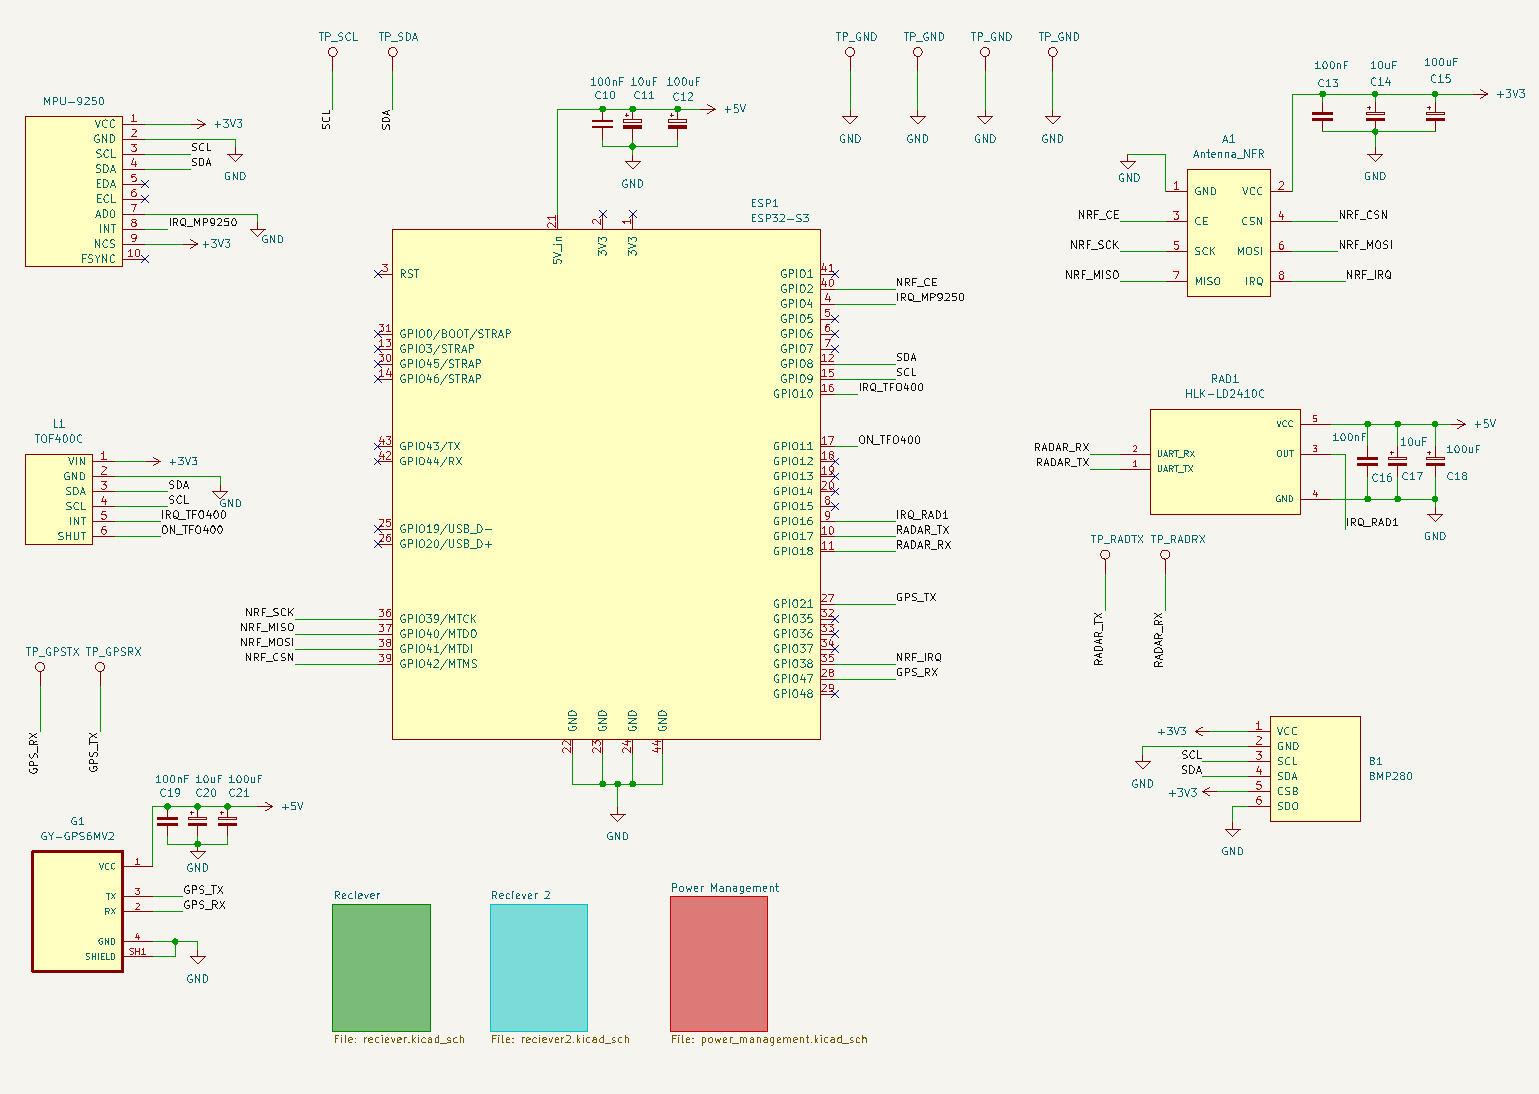
\includegraphics[width=\linewidth]{Figures/transmitter_schematic.pdf}
    \caption{Esquema eléctrico completo del nodo transmisor}
    \label{fig:esquema_kicad_trans}
\end{figure}


\subsection{Nodo receptor}
El nodo receptor se limita al ESP32-C3 Super Mini y al transceptor NRF24L01+, comunicados por SPI, como se muestra en la \cref{fig:esquema_kicad_rec}. Los condensadores de \textit{bulk} situados junto al módulo de radio estabilizan su alimentación durante la recepción.
\begin{figure}[H]
    \centering
    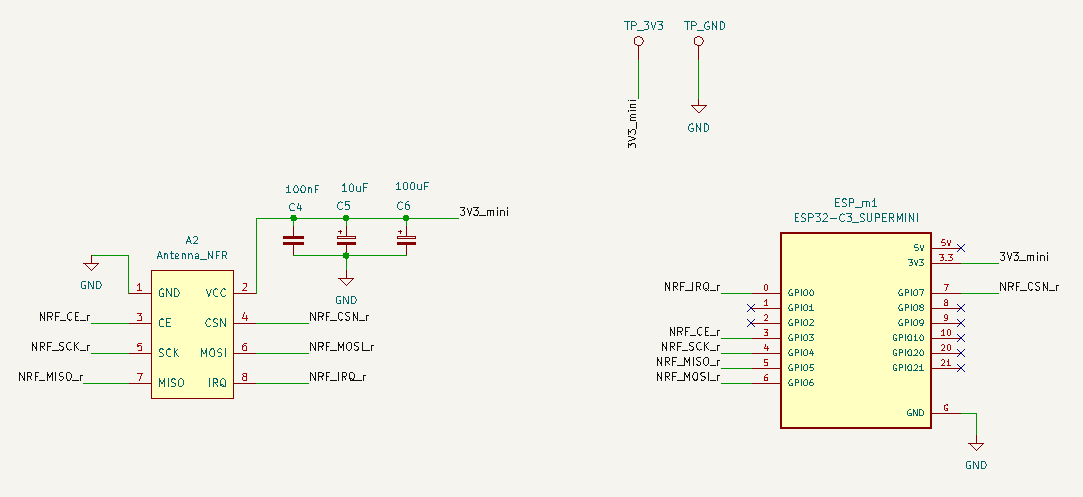
\includegraphics[width=\linewidth]{Figures/reciever_schematic.pdf}
    \caption{Esquema eléctrico completo del nodo receptor}
    \label{fig:esquema_kicad_rec}
\end{figure}

\subsection{Alimentación}
El subsistema de alimentación obtiene el raíl de \SI{5}{\volt} del conector USB-C y genera el de \SI{3.3}{\volt} mediante el LDO NJM12856DL3, como se muestra en la \cref{fig:esquema_kicad_alimentacion}. Los condensadores de desacoplo asociados al regulador son los descritos en la \cref{sec:caps_desacoplo}.
\begin{figure}[H]
    \centering
    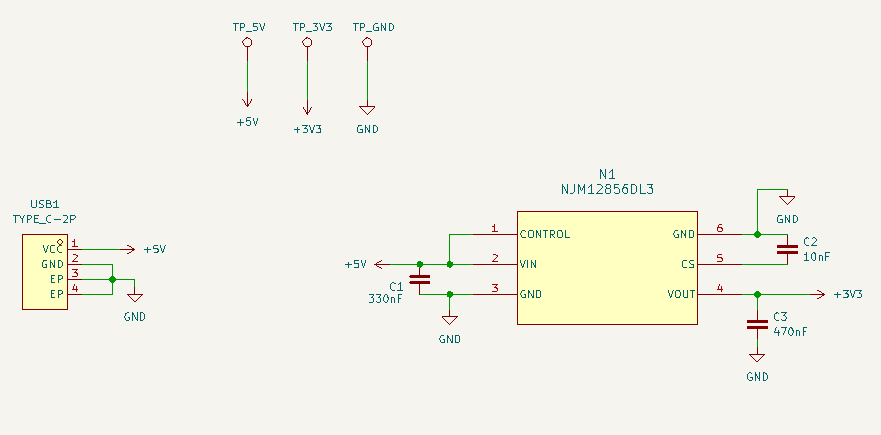
\includegraphics[width=\linewidth]{Figures/power_schematic.pdf}
    \caption{Esquema eléctrico completo del sistema de alimentación}
    \label{fig:esquema_kicad_alimentacion}
\end{figure}


\subsection{Asignación de pines del transmisor}
\label{sec:pines_tx}

La asignación de pines del ESP32-S3 a cada función se resume en la
\cref{tab:pines_tx}. El detalle de todos los pines se puede ver en el esquema eléctrico de la \cref{fig:esquema_kicad_trans}.

\begin{table}[H]
    \centering
    \caption{Asignación de pines del ESP32-S3 (nodo transmisor)}
    \label{tab:pines_tx}
    \footnotesize
    \begin{tabularx}{\linewidth}{l l X}
        \toprule
        \textbf{GPIO} & \textbf{Función} & \textbf{Componente} \\
        \midrule
        GPIO8  & I2C SDA   & MPU-9250, BMP280, VL53L1X \\
        GPIO9  & I2C SCL   & MPU-9250, BMP280, VL53L1X \\
        GPIO21 & UART1 RX  & NEO-6M (TX) \\
        GPIO47 & UART1 TX  & NEO-6M (RX) \\
        GPIO17 & UART2 RX  & HLK-LD2410C (TX) \\
        GPIO18 & UART2 TX  & HLK-LD2410C (RX) \\
        GPIO41 & SPI MOSI  & NRF24L01+ \\
        GPIO40 & SPI MISO  & NRF24L01+ \\
        GPIO39 & SPI SCK   & NRF24L01+ \\
        GPIO42 & SPI CSN   & NRF24L01+ \\
        GPIO2  & GPIO CE   & NRF24L01+ \\
        \bottomrule
    \end{tabularx}
\end{table}

\subsection{Bus I2C: pull-ups y direccionamiento}
\label{sec:bus_i2c}

Los tres sensores I2C no presentan ningún conflicto de direcciones, el MPU-9250 ocupa
\texttt{0x68} con AD0 a GND \cite{ps_mpu9250}, el BMP280 \texttt{0x76}
\cite{ds_bmp280} y el VL53L1X \texttt{0x29} por defecto \cite{ds_vl53l1x}. Por último, el
magnetómetro AK8963 integrado en el MPU-9250 se accede en \texttt{0x0C}
mediante el modo \textit{bypass} del MPU \cite{mpu9250_regmap}.

En cuanto a las resistencias de pull-up, cada módulo \textit{breakout} incluye su propia
pareja de resistencias en SDA y SCL (\SI{10}{\kilo\ohm} hacia
VCC). Al conectar tres módulos en paralelo, la resistencia equivalente cae a
aproximadamente \SI{3.3}{\kilo\ohm}, valor que cae dentro de los límites
recomendados por la especificación I2C de NXP \cite{nxp_i2c} para velocidades
estándar y rápida. Aun así, en el \cref{ch:validacion} se confirma que no hay problemas en el bus.


\subsection{Asignación de pines del receptor}
\label{sec:pines_rx}

El nodo receptor utiliza un ESP32-C3 Super Mini cuyo único componente externo
es el transceptor NRF24L01+ comunicado por SPI (\cref{tab:pines_rx}). El pin
GPIO8 se reserva para el LED \textit{onboard}. La comunicación con el PC se realiza con el conector USB-C nativo
del ESP32-C3 mediante USB-CDC.

\begin{table}[H]
    \centering
    \caption{Asignación de pines del ESP32-C3 Super Mini (nodo receptor)}
    \label{tab:pines_rx}
    \footnotesize
    \begin{tabularx}{\linewidth}{l l X}
        \toprule
        \textbf{GPIO} & \textbf{Función} & \textbf{Notas} \\
        \midrule
        GPIO4 & SPI SCK  & NRF24L01+ \\
        GPIO5 & SPI MISO & NRF24L01+ \\
        GPIO6 & SPI MOSI & NRF24L01+ \\
        GPIO7 & SPI CSN  & NRF24L01+ \\
        GPIO3 & GPIO CE  & NRF24L01+ \\
        GPIO8 & LED      & Onboard \\
        \bottomrule
    \end{tabularx}
\end{table}


\section{Diseño físico de la PCB}
\label{sec:layout}

El diseño físico se ha realizado en KiCad \cite{kicad_pcbnew} sobre una PCB de
dos capas con dimensiones de 180 $\times$ \SI{115}{\milli\meter}. La capa superior
concentra la mayor parte de las señales y rutas de corriente, mientras que la
capa inferior se rellena como plano de masa continuo, con las mínimas trazas posibles, para garantizar la
integridad de señal y reducir las interferencias electromagnéticas. También se ha rellenado la capa superior con masa para mejorar la integridad de la señal y asegurar un retorno correcto de las señales.

\subsection{Restricciones críticas de layout}
\label{sec:layout_restricciones}

Se han aplicado tres restricciones críticas en la disposición de componentes:

\begin{itemize}
    \item \textbf{Keepout de la antena del ESP32-S3.} Se reserva un área sin
    cobre de \SI{15}{\milli\meter} alrededor de la antena PCB del módulo en
    ambas capas, conforme a las recomendaciones del fabricante
    \cite{ds_esp32s3}.

    \item \textbf{Separación entre el radar y la IMU.} El HLK-LD2410C
    transmite a \SI{24}{\giga\hertz} y la IMU es sensible a vibraciones y
    perturbaciones electromagnéticas, por esto se mantienen separados al menos
    \SI{15}{\milli\meter} para minimizar el acoplamiento.

    \item \textbf{Antena del GPS orientada al borde.} El NEO-6M se ubica en
    un borde de la PCB con la antena cerámica hacia el exterior, evitando
    obstáculos metálicos que degradarían la recepción satelital. También se ha dejado un área sin masa alrededor de la antena para minimizar interferencias.
\end{itemize}

\newpage

\subsection{Anchura de pistas y nodo receptor}
\label{sec:layout_pistas}

Se definen dos clases de redes principales con anchuras diferenciadas: \SI{0.25}{\milli
\meter} para señales de baja corriente (I2C, UART, SPI, GPIO) y \SI{1}{
\milli\meter} para las rutas de alimentación. Como se ha mencionado anteriormente, el plano de
masa de la capa inferior se cose a la capa superior mediante un conjunto de
vías distribuidas, reforzando el camino de retorno de las señales.

En cuanto a la PCB del receptor, se ha tomado la decisión de integrar la PCB como una pestaña separable en un borde de la PCB principal, unida mediante pequeñas secciones de PCB. Esto hace que se pueda fabricar ambas PCB en una misma orden de producción, reduciendo el coste global.

En las siguientes figuras se puede ver el diseño de la PCB en el software, y el renderizado 3D final de cómo debería quedar.

\begin{figure}[H]
    \centering
    \includegraphics[width=\linewidth]{Figures/front_pcb_kicad.png}
    \caption{Diseño de la cara superior de la PCB}
    \label{fig:front_pcb_design}
\end{figure}

\begin{figure}[H]
    \centering
    \includegraphics[width=\linewidth]{Figures/back_pcb_kicad.png}
    \caption{Diseño del reverso de la PCB}
    \label{fig:back_pcb_design}
\end{figure}


\begin{figure}[H]
    \centering
    \includegraphics[width=\linewidth]{Figures/iso_pcb.png}
    \caption{Render 3D de la PCB}
    \label{fig:pcb_layout}
\end{figure}

\newpage
\section{Fabricación y ensamblaje}
\label{sec:fabricacion}

La PCB se ha fabricado mediante el servicio JLCPCB, seleccionado por su coste
competitivo (RC01) y su buena calidad. Las especificaciones de fabricación se resumen en la \cref{tab:pcb_fab}.

\begin{table}[H]
    \centering
    \caption{Especificaciones de fabricación de la PCB}
    \label{tab:pcb_fab}
    \footnotesize
    \begin{tabularx}{0.75\linewidth}{l X}
        \toprule
        \textbf{Parámetro} & \textbf{Valor} \\
        \midrule
        % TODO: confirma los valores reales que pediste en JLCPCB
        Fabricante           & JLCPCB \\
        Número de capas      & 2 \\
        Dimensiones          & 180 $\times$ \SI{115}{\milli\meter} \\
        Espesor              & \SI{1.6}{\milli\meter} \\
        Grosor de cobre      & 1~oz (\SI{35}{\micro\meter}) \\
        Acabado superficial  & HASL \\
        \bottomrule
    \end{tabularx}
\end{table}


\begin{figure}[H]
    \centering
    \begin{subfigure}[b]{0.45\linewidth}
        \centering
        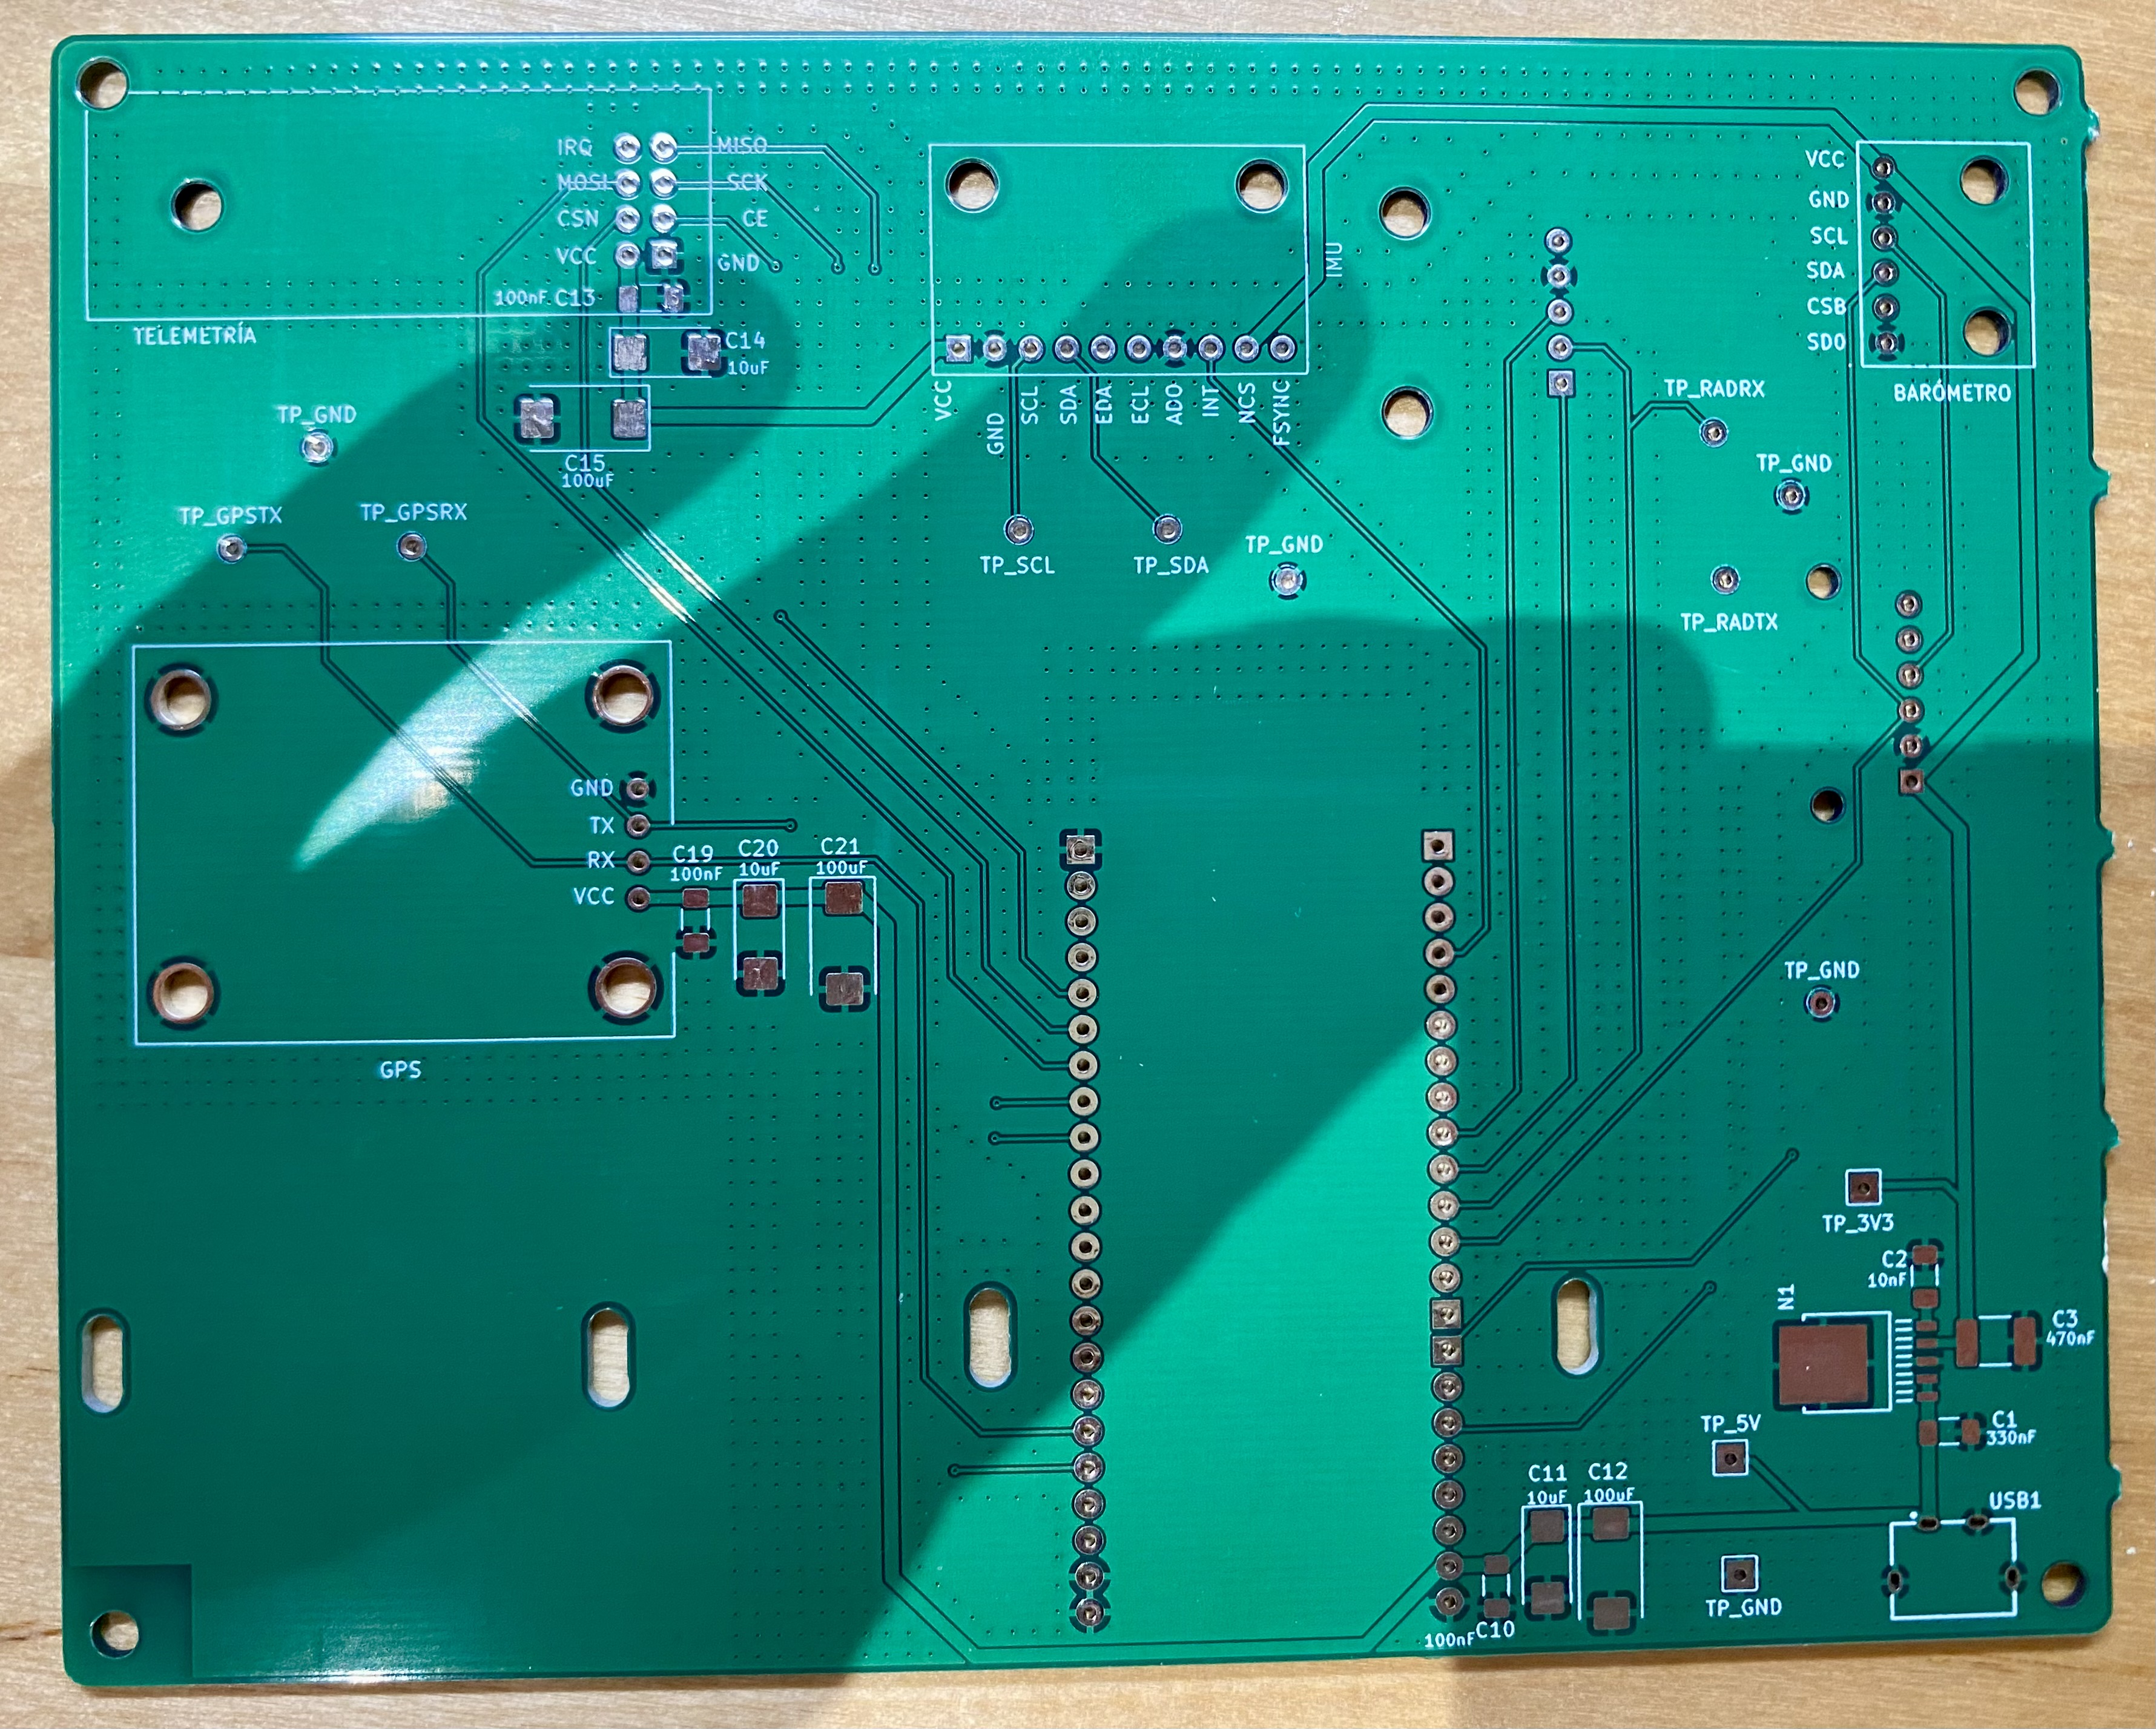
\includegraphics[width=\linewidth]{Figures/front_pcb.jpeg}
        \caption{Cara superior de la PCB}
        \label{fig:cara_pcb_fabricada}
    \end{subfigure}
    \hfill
    \begin{subfigure}[b]{0.45\linewidth}
        \centering
        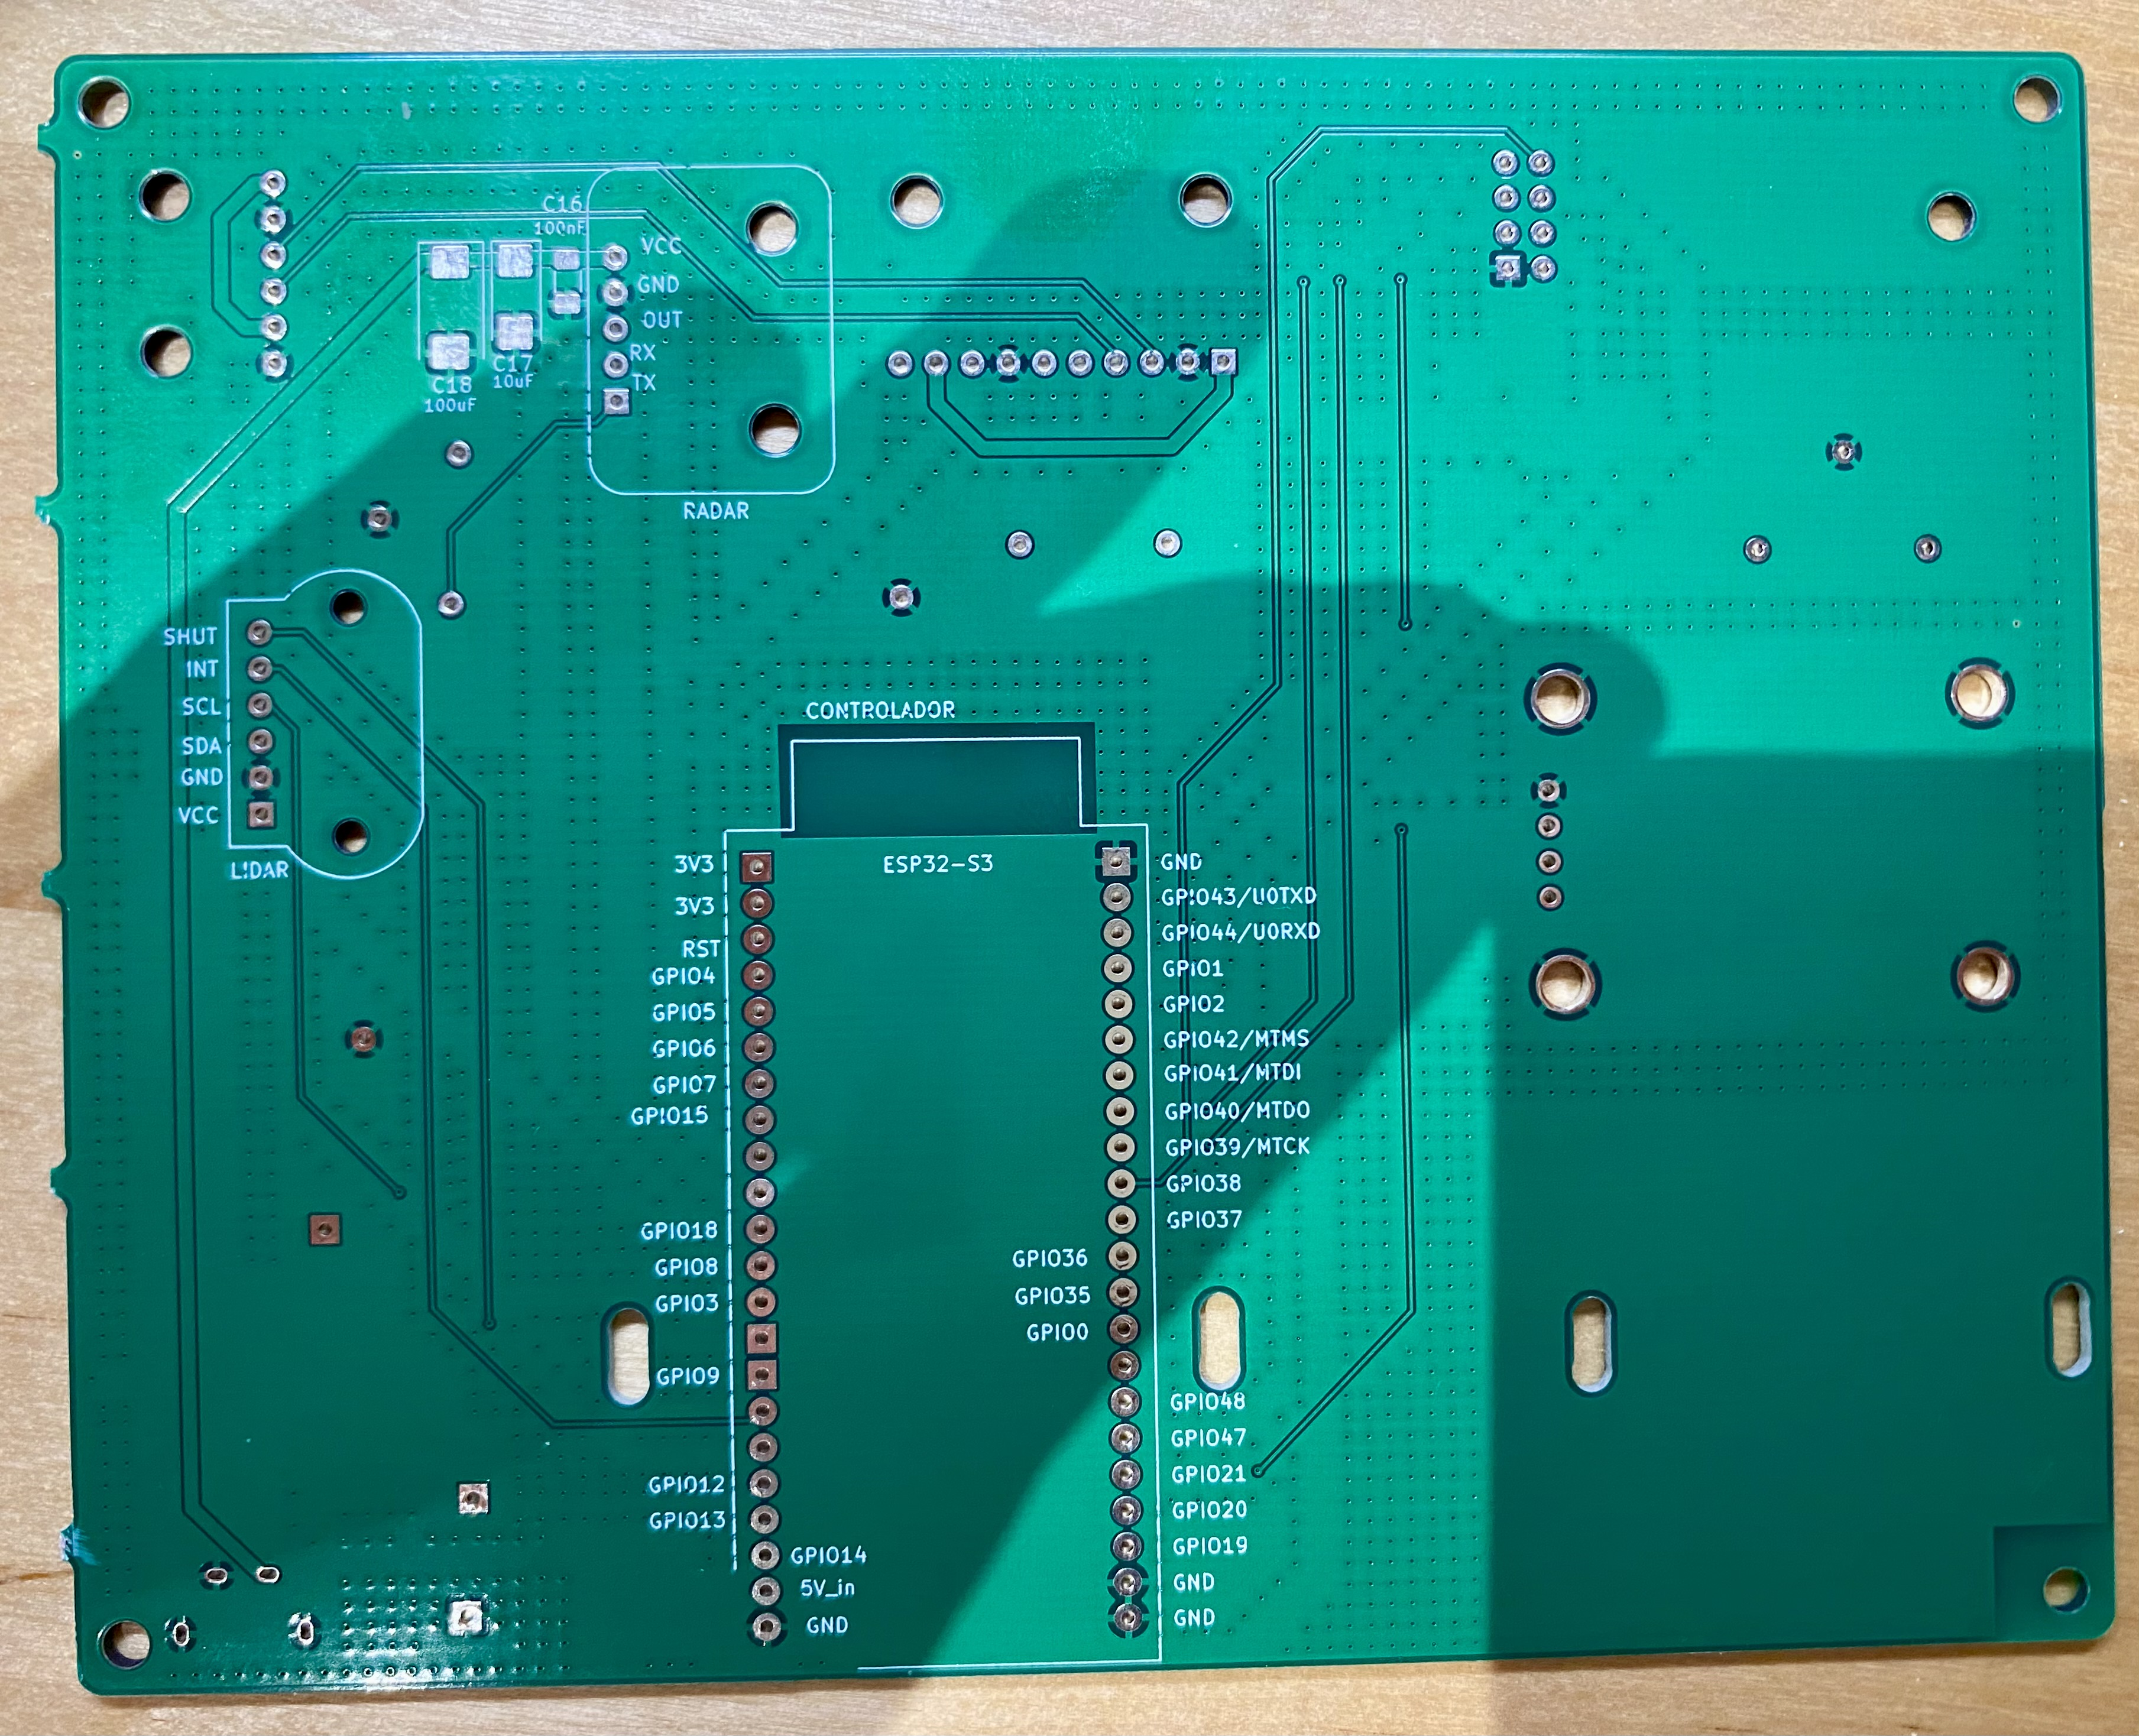
\includegraphics[width=\linewidth]{Figures/back_pcb.jpeg}
        \caption{Reverso de la PCB}
        \label{fig:reverso_pcb_fabricada}
    \end{subfigure}
    \caption{PCB del nodo transmisor antes de incorporar ningún componente}
    \label{fig:transmitter_pcb}
\end{figure}
\begin{figure}[H]
    \centering
    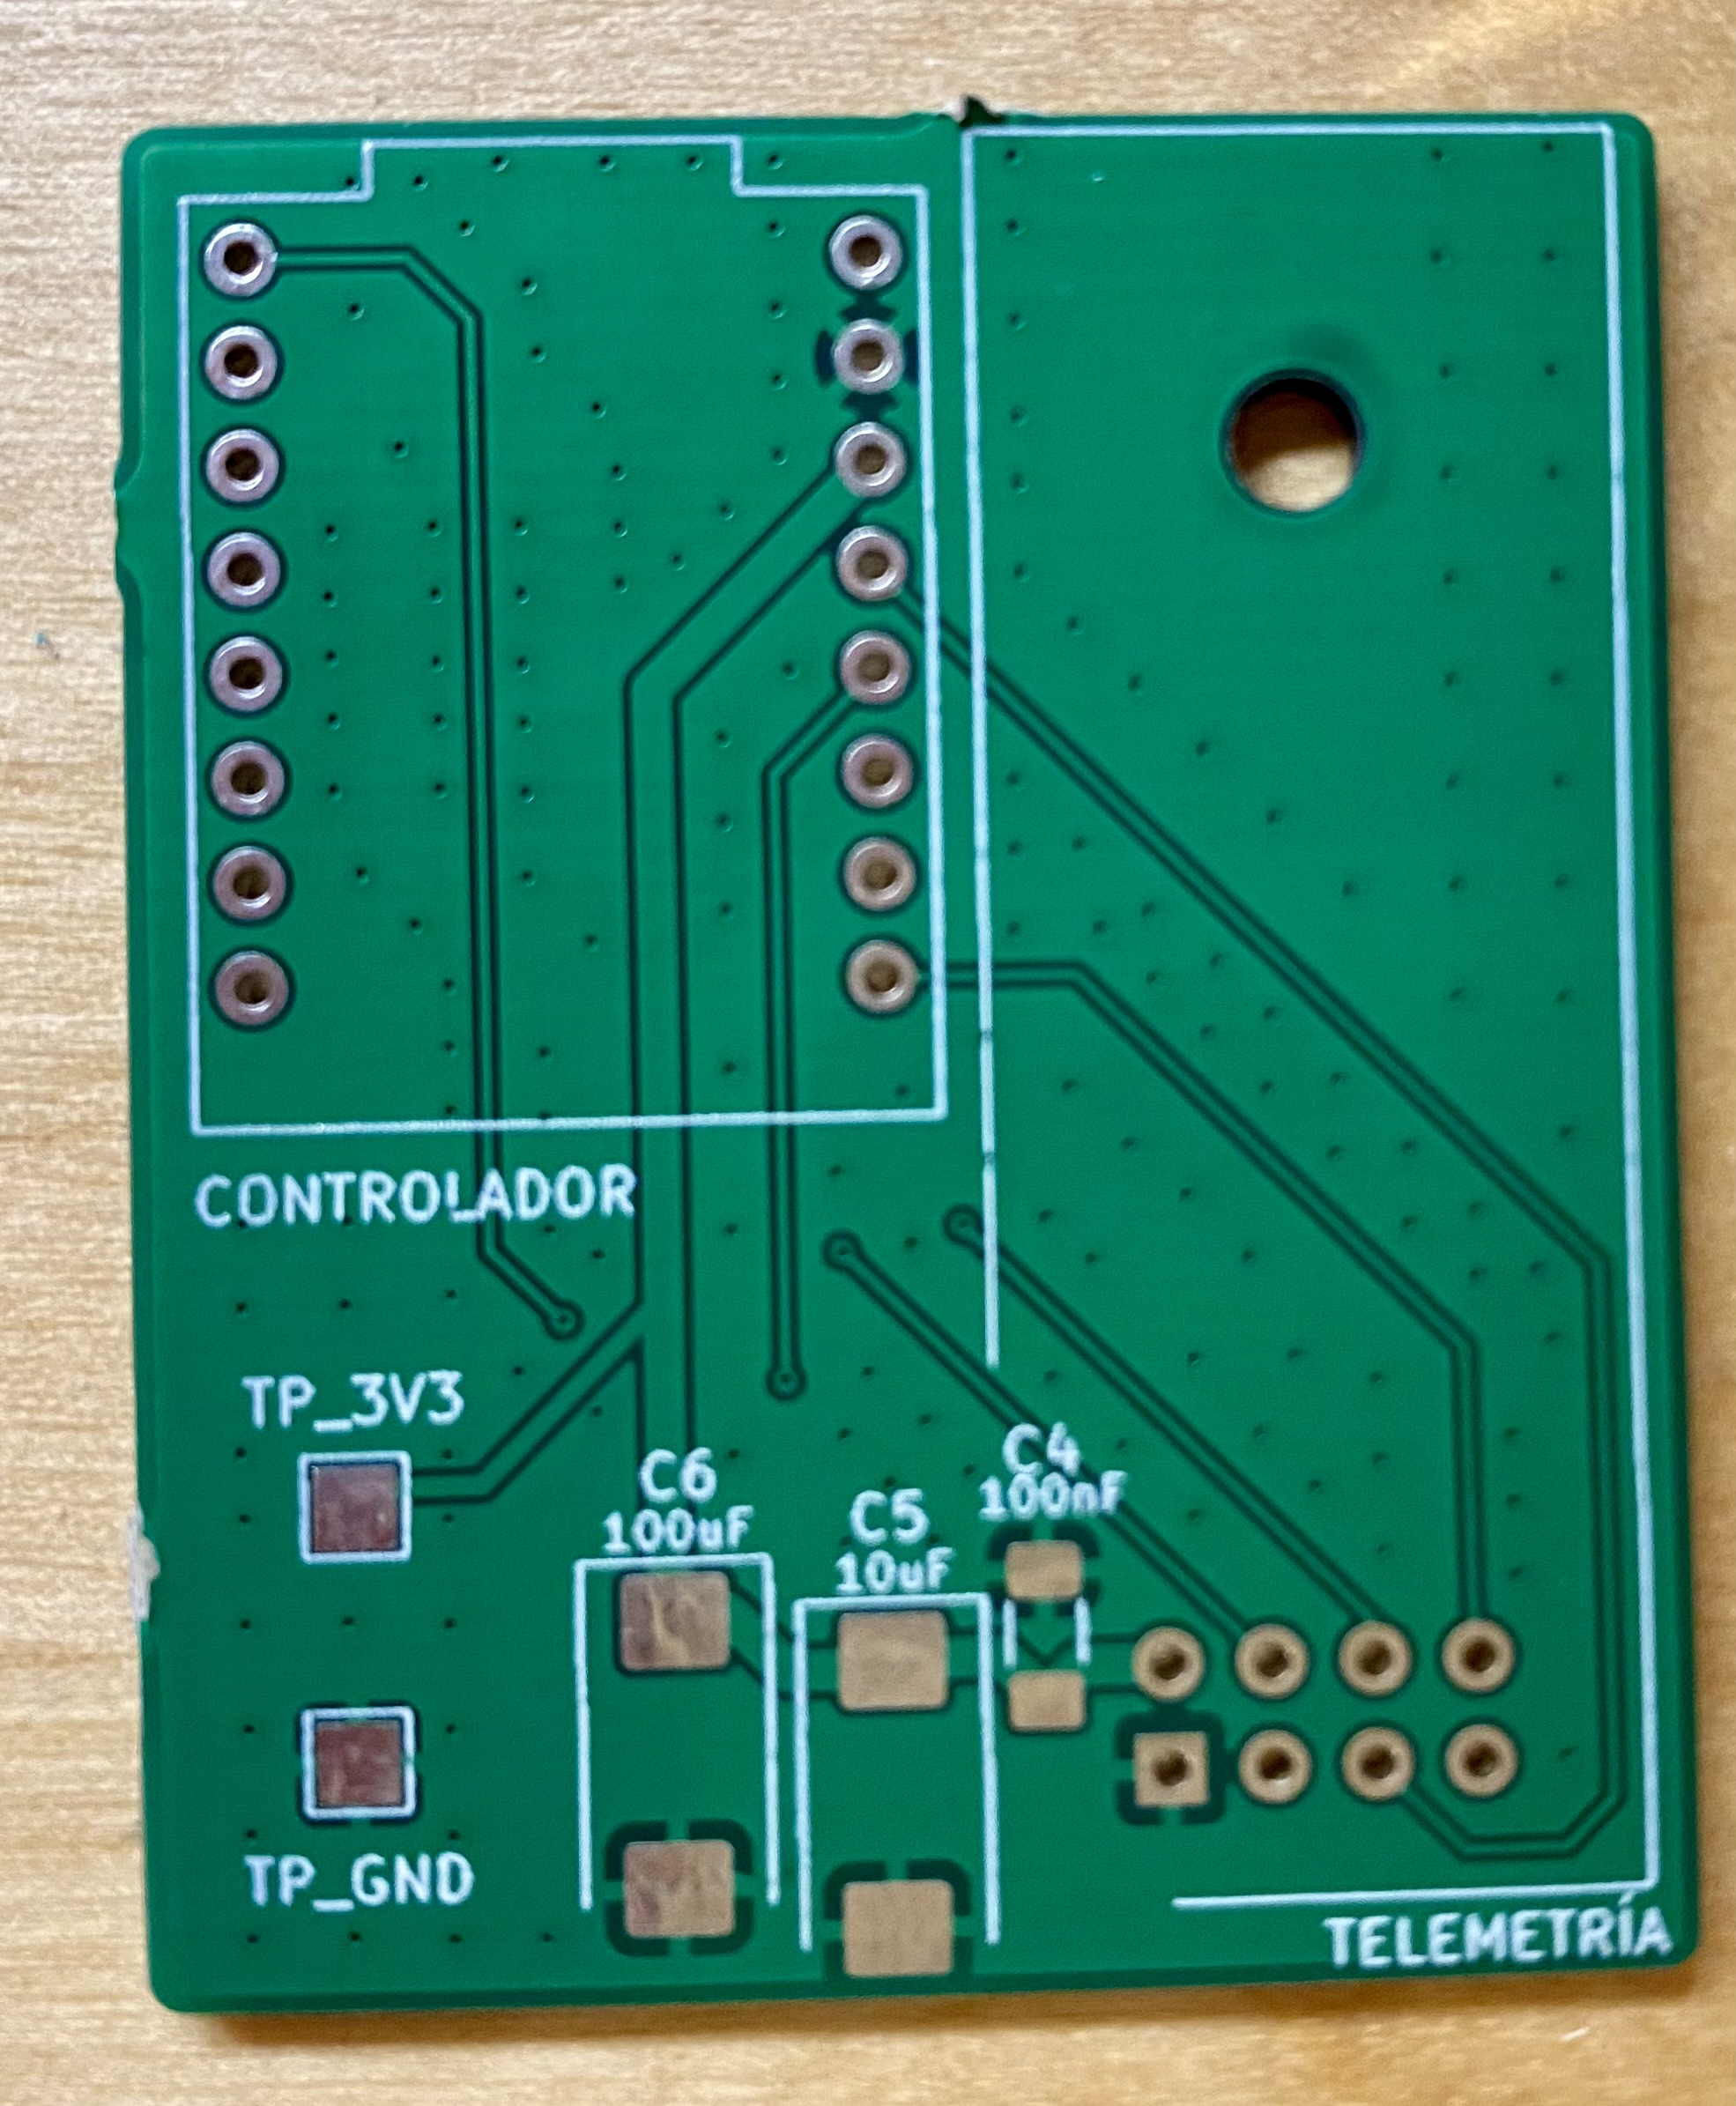
\includegraphics[width=0.35\textwidth]{Figures/reciever_pcb.jpeg}
    \caption{PCB del nodo receptor antes de incorporar ningún componente}
    \label{fig:reciever_pcb}
\end{figure}

Una vez obtenida la PCB, primero se verifica que no hay ningún defecto a simple vista antes de proceder al ensamblaje, y luego se separa el receptor de la PCB principal. El ensamblaje se realiza de forma manual mediante soldador convencional. Los componentes pasivos en formato SMD se sueldan primero, seguidos
del LDO, el conector USB-C y, por último los zócalos hembra para los módulos
\textit{breakout}. La elección de zócalos en lugar de soldadura directa de los componentes a la PCB permite sustituir los módulos durante el desarrollo y reutilizarlos en futuras iteraciones, además de facilitar la sustitución en caso de fallo de algún componente.

\begin{figure}[H]
    \centering
    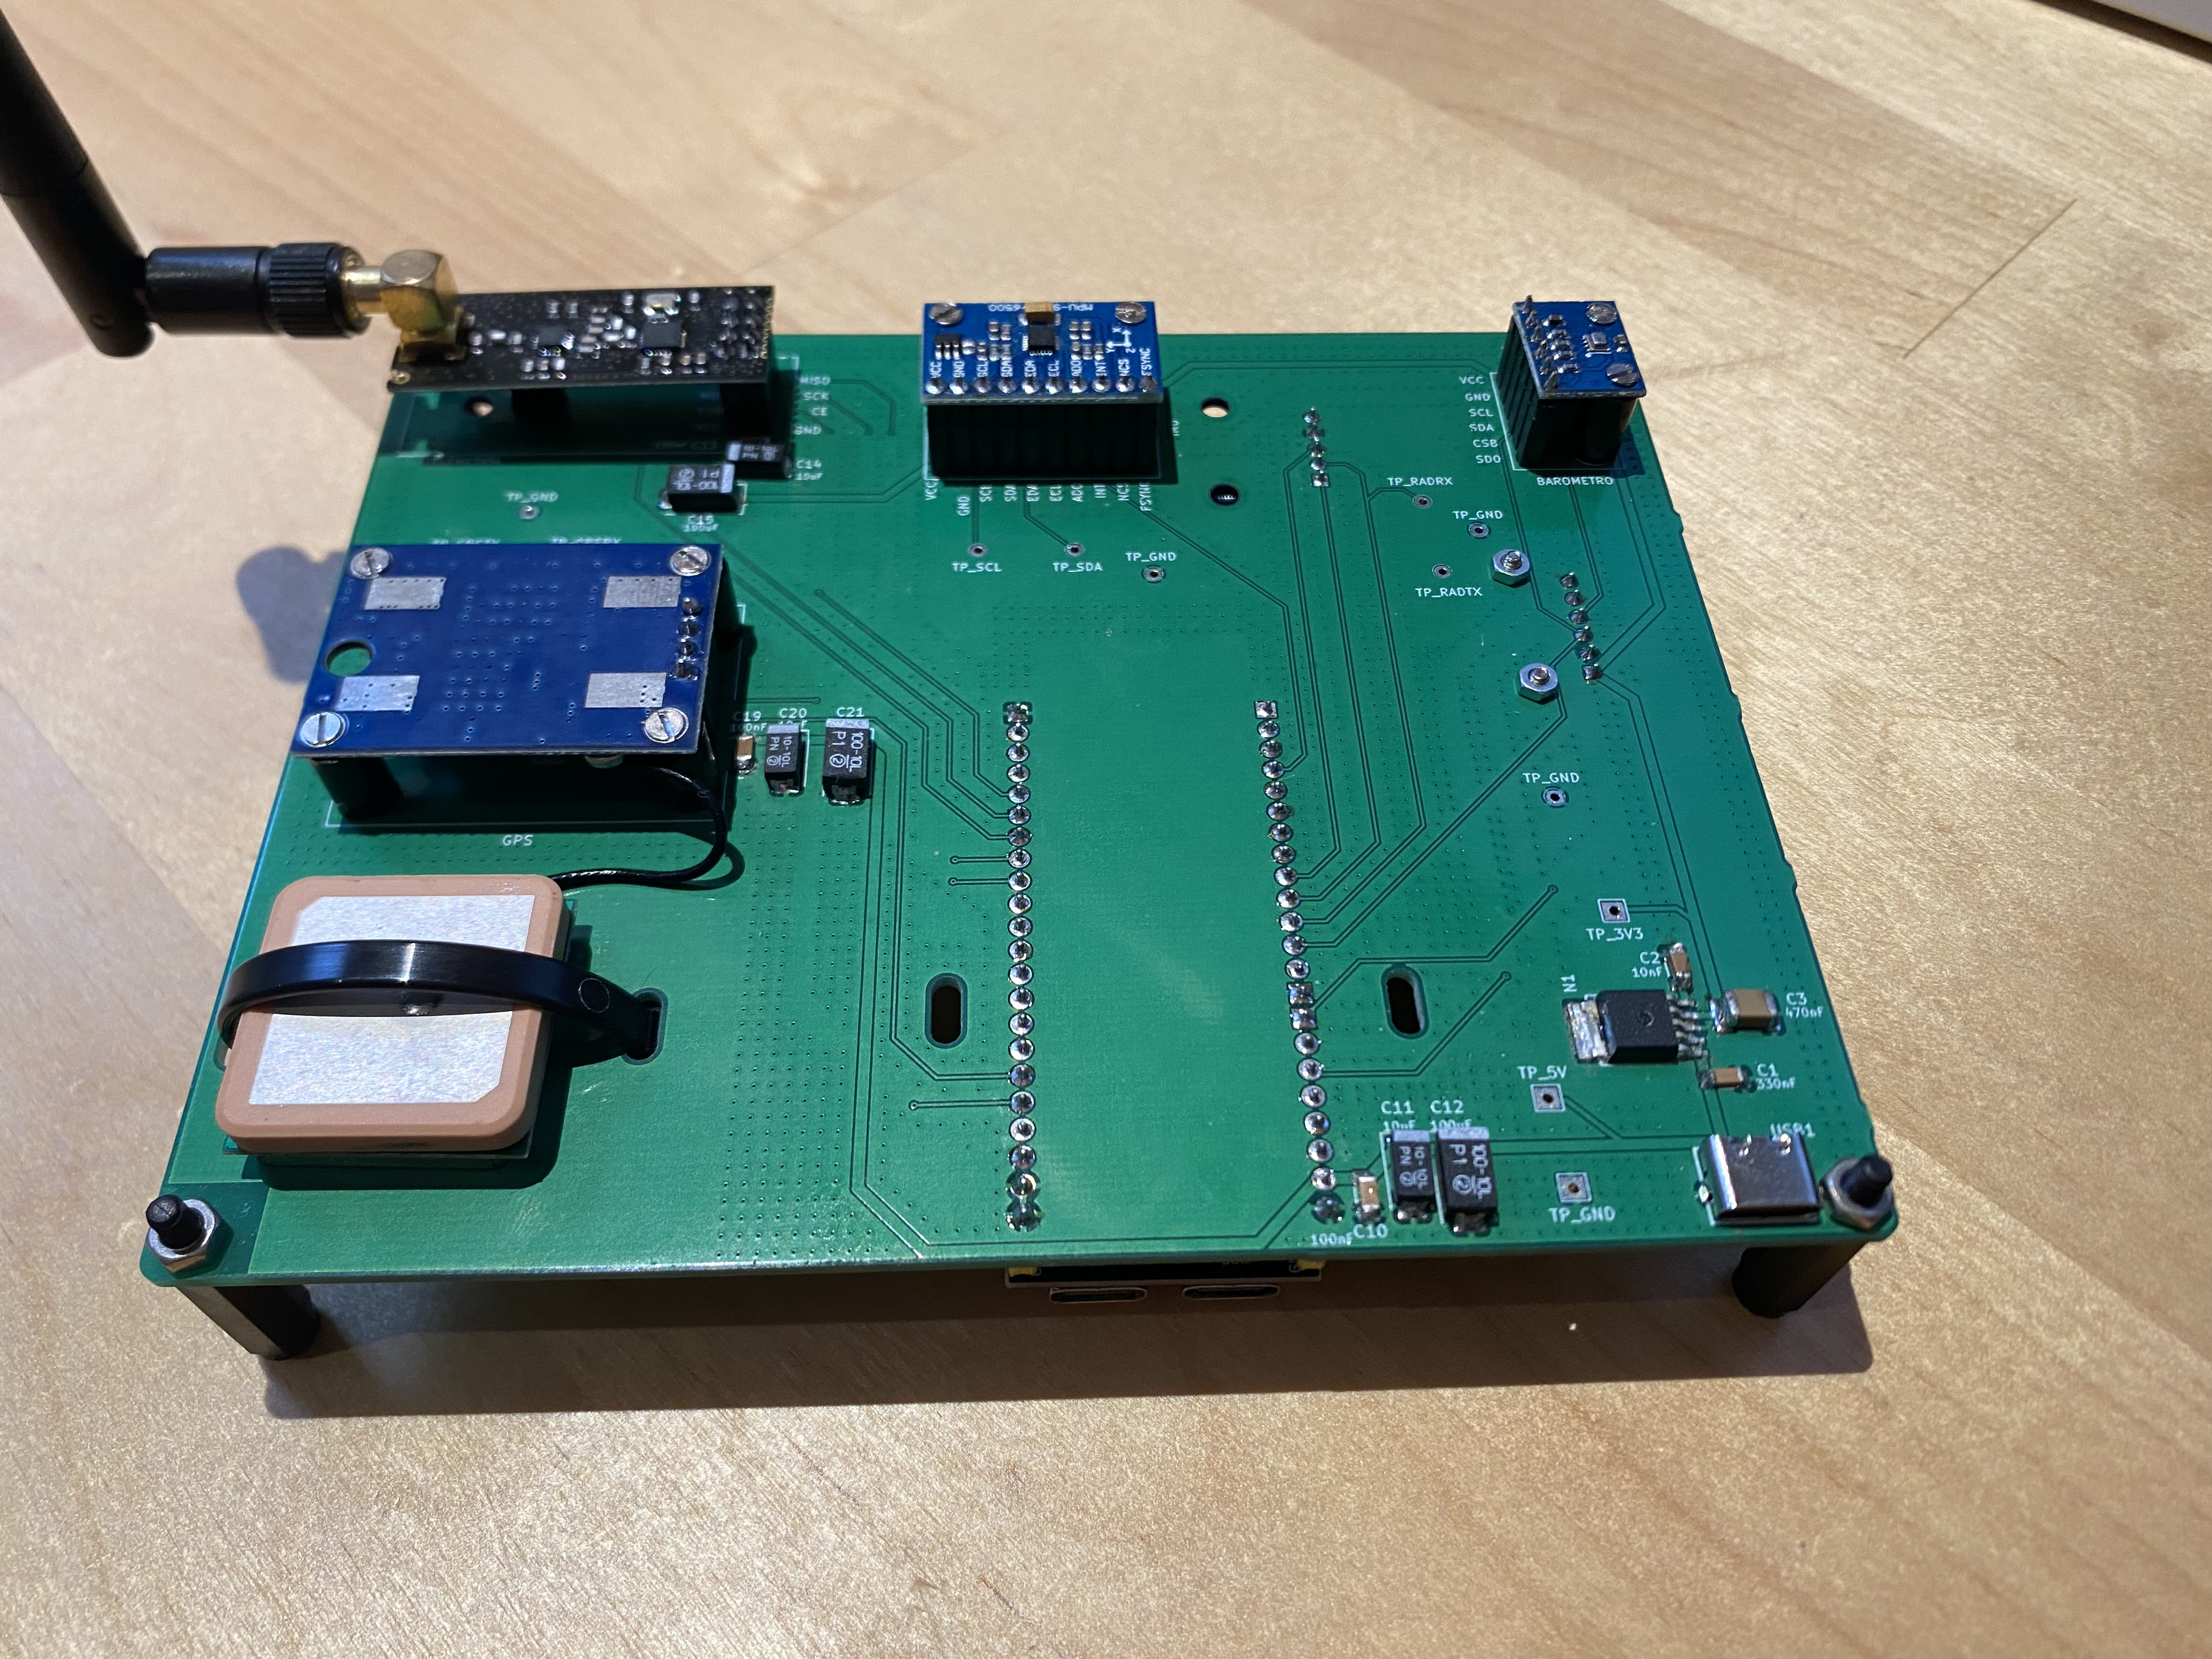
\includegraphics[width=0.70\linewidth]{Figures/real_pcb.jpeg}
    \caption{PCB del nodo transmisor totalmente ensamblada con todos los
    módulos incorporados}
    \label{fig:pcb_ensamblado}
\end{figure}

\begin{figure}[H]
    \centering
    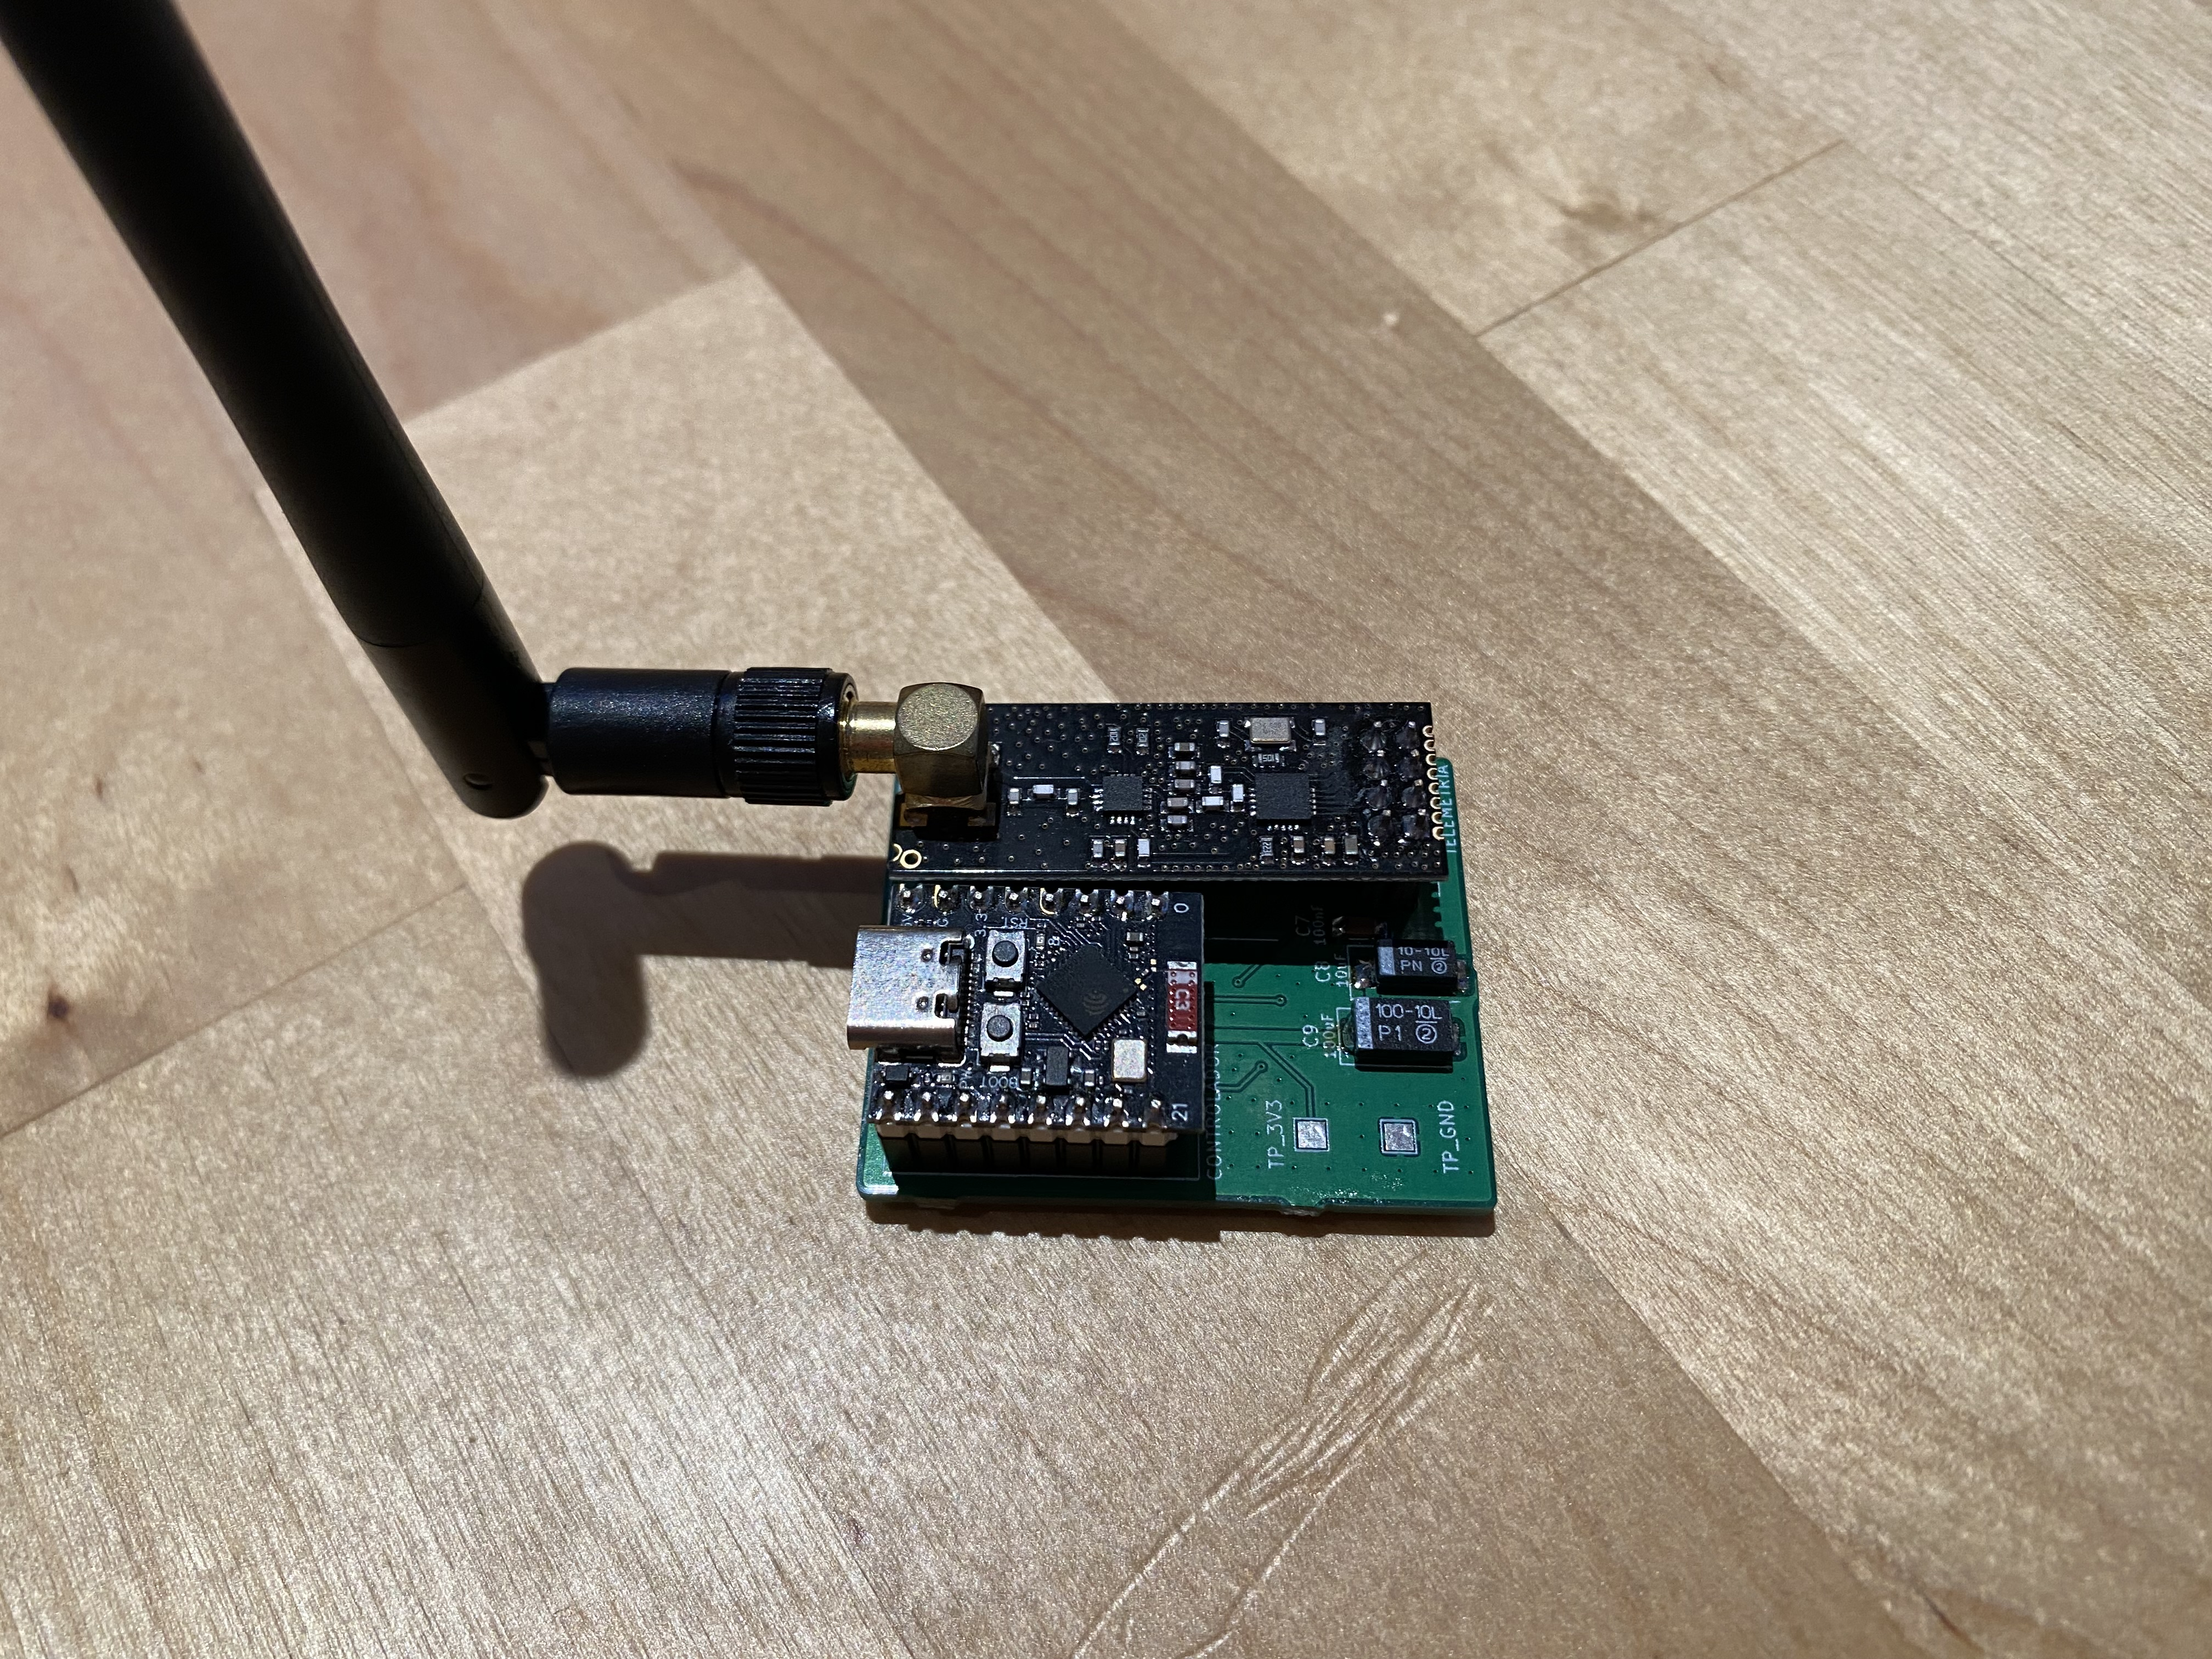
\includegraphics[width=0.70\linewidth]{Figures/real_reciever_pcb.jpeg}
    \caption{PCB del nodo receptor totalmente ensamblada con todos los
    módulos incorporados}
    \label{fig:pcb__receptor_ensamblado}
\end{figure}

El coste total del sistema, incluyendo fabricación de la PCB, componentes
pasivos y módulos \textit{breakout}, se desglosa en la \cref{tab:bom_resumen}
de la \cref{sec:sel_resumen}.

\section{Verificación del hardware}
\label{sec:verificacion}

Antes de cargar el firmware se realizaron dos pruebas de \textit{bring-up}
sobre la PCB. Primero, una verificación de continuidad con el multímetro y
la placa sin alimentar, contrastando las \textit{nets} contra el
\textit{netlist} del esquemático y descartando cortocircuitos entre los
planos de alimentación y masa, para asegurar que no había cortocircuitos producidos en el proceso de soldadura. No se detectaron circuitos abiertos ni cortocircuitos. Después, ya con la
placa alimentada por USB-C y sin carga, se midieron los \textit{rails} de
\SI{5}{\volt} y \SI{3.3}{\volt}, que quedaron dentro de las tolerancias del
regulador NJM12856DL3 \cite{ds_njm12856}. Al final se confirmó el funcionamiento correcto de todos los módulos del sistema.